\documentclass[a4paper,14pt]{report}
\usepackage[utf8]{inputenc}
\usepackage[ukrainian]{babel}
\usepackage{amsmath,amsfonts,amssymb}
\usepackage{graphicx}
\usepackage{geometry}
\usepackage{fancyhdr}
\usepackage{titlesec}
\usepackage{indentfirst}
\usepackage{caption}
\usepackage{listings}
\usepackage{hyperref}
\usepackage{float}
\usepackage{tocloft}
\usepackage{enumitem}
\usepackage{pdfpages} % для вставки титульного аркуша, якщо він як PDF

\graphicspath{ {./img/} }


\geometry{left=3cm, right=1.5cm, top=2cm, bottom=2cm}
\setlength{\parindent}{1.25cm}
\setlength{\parskip}{0.5em}

% Стилі заголовків
\titleformat{\section}{\Large\bfseries\centering}{РОЗДІЛ \thesection.}{1em}{\MakeUppercase}
\titleformat{\subsection}{\normalsize\bfseries}{\thesubsection.}{0.5em}{}

% Стиль для змісту
\renewcommand{\cftsecleader}{\cftdotfill{\cftdotsep}}
\usepackage{titlesec}
\titleformat{\section}[block]{\center\normalfont\Large\bfseries}{\thesection}{1em}{}

\def\changemargin#1#2{\list{}{\rightmargin#2\leftmargin#1}\item[]}
\let\endchangemargin=\endlist 
\makeatletter
\def\@makechapterhead#1{%
  %\vspace*{50\p@}%
  {\parindent \z@ \raggedright \normalfont
    \ifnum \c@secnumdepth >\m@ne
      \if@mainmatter
        %\huge\bfseries \@chapapp\space \thechapter
        \center\Huge\bfseries \thechapter.\space%
        %\par\nobreak
        %\vskip 20\p@
      \fi
    \fi
    \interlinepenalty\@M
    \Huge \bfseries #1\par\nobreak
    \vskip 40\p@
  }}
\makeatother

\begin{document}

\begin{center}
    \normalsize
    НАЦІОНАЛЬНИЙ ТЕХНІЧНИЙ УНІВЕРСИТЕТ УКРАЇНИ \\
    «КИЇВСЬКИЙ ПОЛІТЕХНІЧНИЙ ІНСТИТУТ імені Ігоря СІКОРСЬКОГО» \\
    Навчально-науковий Фізико-технічний інститут
\end{center}

\vspace*{4cm} % Вертикальний відступ від верхнього блоку до назви роботи

% Центральний блок (Назва роботи)
\begin{center}
    \Large \textbf{РОЗРАХУНКОВО-ГРАФІЧНА РОБОТА} \\
    \normalsize з кредитного модуля «Інтелектуальні обчислення» \\
    на тему: \\
    \textbf{"РОЗПІЗНАВАННЯ РОБОЧОЇ ПОВЕРХНІ СТОЛУ 3D ПРИНТЕРА ПРЯМИМИ ТА ІТЕРАЦІЙНИМИ МЕТОДАМИ, НЕЙРОННИМИ МЕРЕЖАМИ"} \\
\end{center}

\vspace*{4cm} % Вертикальний відступ від назви роботи до блоку "Виконав"

% Блок "Виконав" (праворуч)
\begin{changemargin}{10cm}{0cm} % Вирівнювання по правому краю
    Виконав: \\
    студент 3 курсу НН ФТІ \\
    Голуб Михайло Вікторович \\
    номер залікової книжки \rule{3cm}{0.4pt} % Лінія для номера залікової книжки
\end{changemargin}

\vspace*{3cm} % Відступ між блоками "Виконав" та "Перевірив"

% Блок "Перевірив" (праворуч)
\begin{changemargin}{10cm}{0cm} % Вирівнювання по правому краю
    Перевірив: \rule{4cm}{0.4pt} \\ \\ % Лінія для підпису
    Оцінка: \rule{4cm}{0.4pt} % Лінія для оцінки
\end{changemargin}

\vfill % Розтягує простір, щоб перемістити наступний вміст до низу сторінки

% Нижній колонтитул
\begin{center}
    Київ-- 2025
\end{center}

\tableofcontents
\newpage

% Розділ "Вступ"
\chapter{Вступ}
\section{Актуальність}
3D принтери технології пошарового наплавлення філаменту (Fused filament fabrication, далі -- FFF 3D принтери) зараз є найбільш поширеними верстатами для швидкого протипування.
Дана технологія має недолік високої кількості браку. Збільшення кількості завчасних зупинок друку через брак може бути досягнуто при використанні методів що використовують контекст (положення друкованого об'єкту в просторі відносно камери), аніж при використанні нейронних мереж які аналізують зображення без жодної додаткової інформації про 3D модель що друкується.
Для розробки і застосування покращених методів необхідно чітко знати положення столу, щоб визначити де на фотографії / відео має знаходитись 3D модель, яка друкується.
Першим кроком з створення таких методів є система розпізнавання робочої поверхні столу FFF 3D принтера.


\section{Мета роботи}
Мета роботи -- побудувати і порівняти методи розпізнавання робочої поверхні столу для FFF 3D принтера Bambulab A1 mini.
\begin{figure}[H]
  \center
  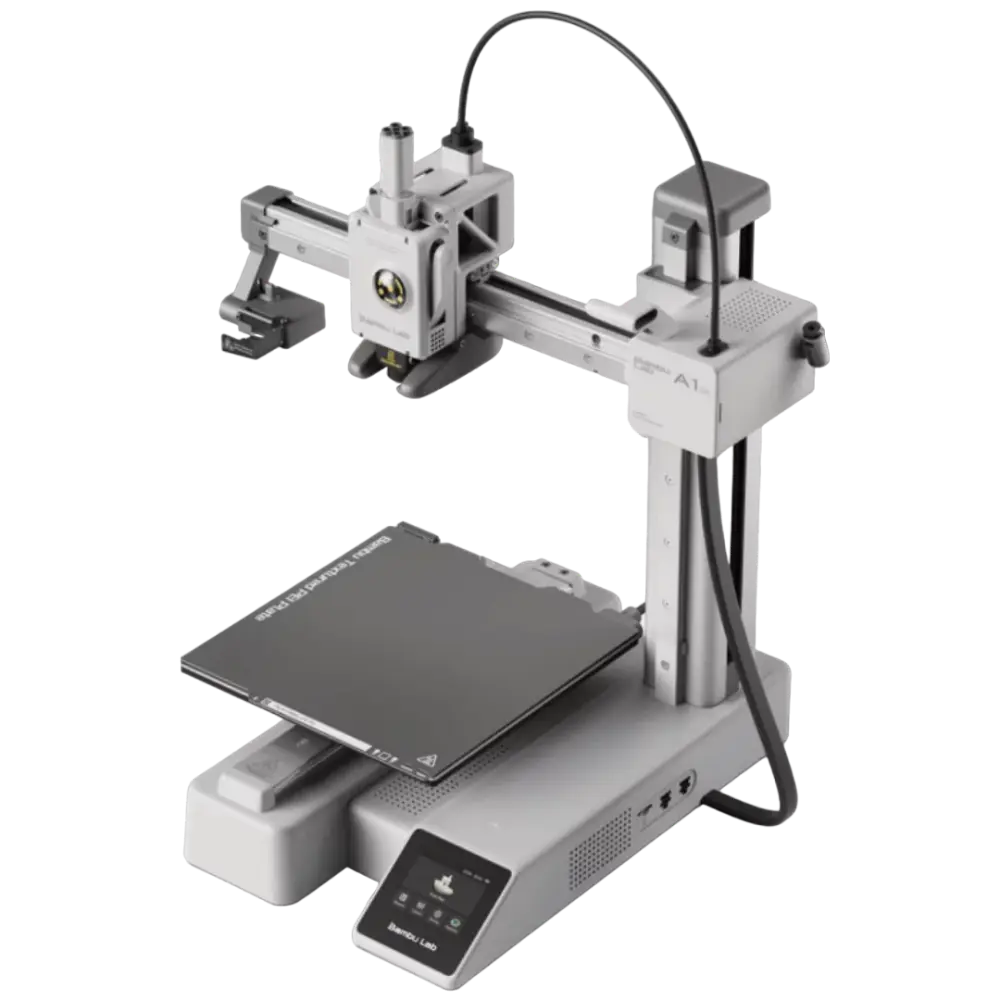
\includegraphics[height=10cm]{a1mini}
  \textbf{\caption{Bambulab A1 mini}}
  \label{fig:a1mini}
\end{figure}

\chapter{Допрограмний етап}
\section{Аналіз об'єкту, що розпізнається}
Необхідно розпізнати робочу поверхню столу FFF 3D принтера Bambulab A1 mini. Дана модель має декілька різних змінних робочих поверхонь, але найбільш розповсюджена -- PEI-пластина.\\
\begin{figure}[H]
  \center
  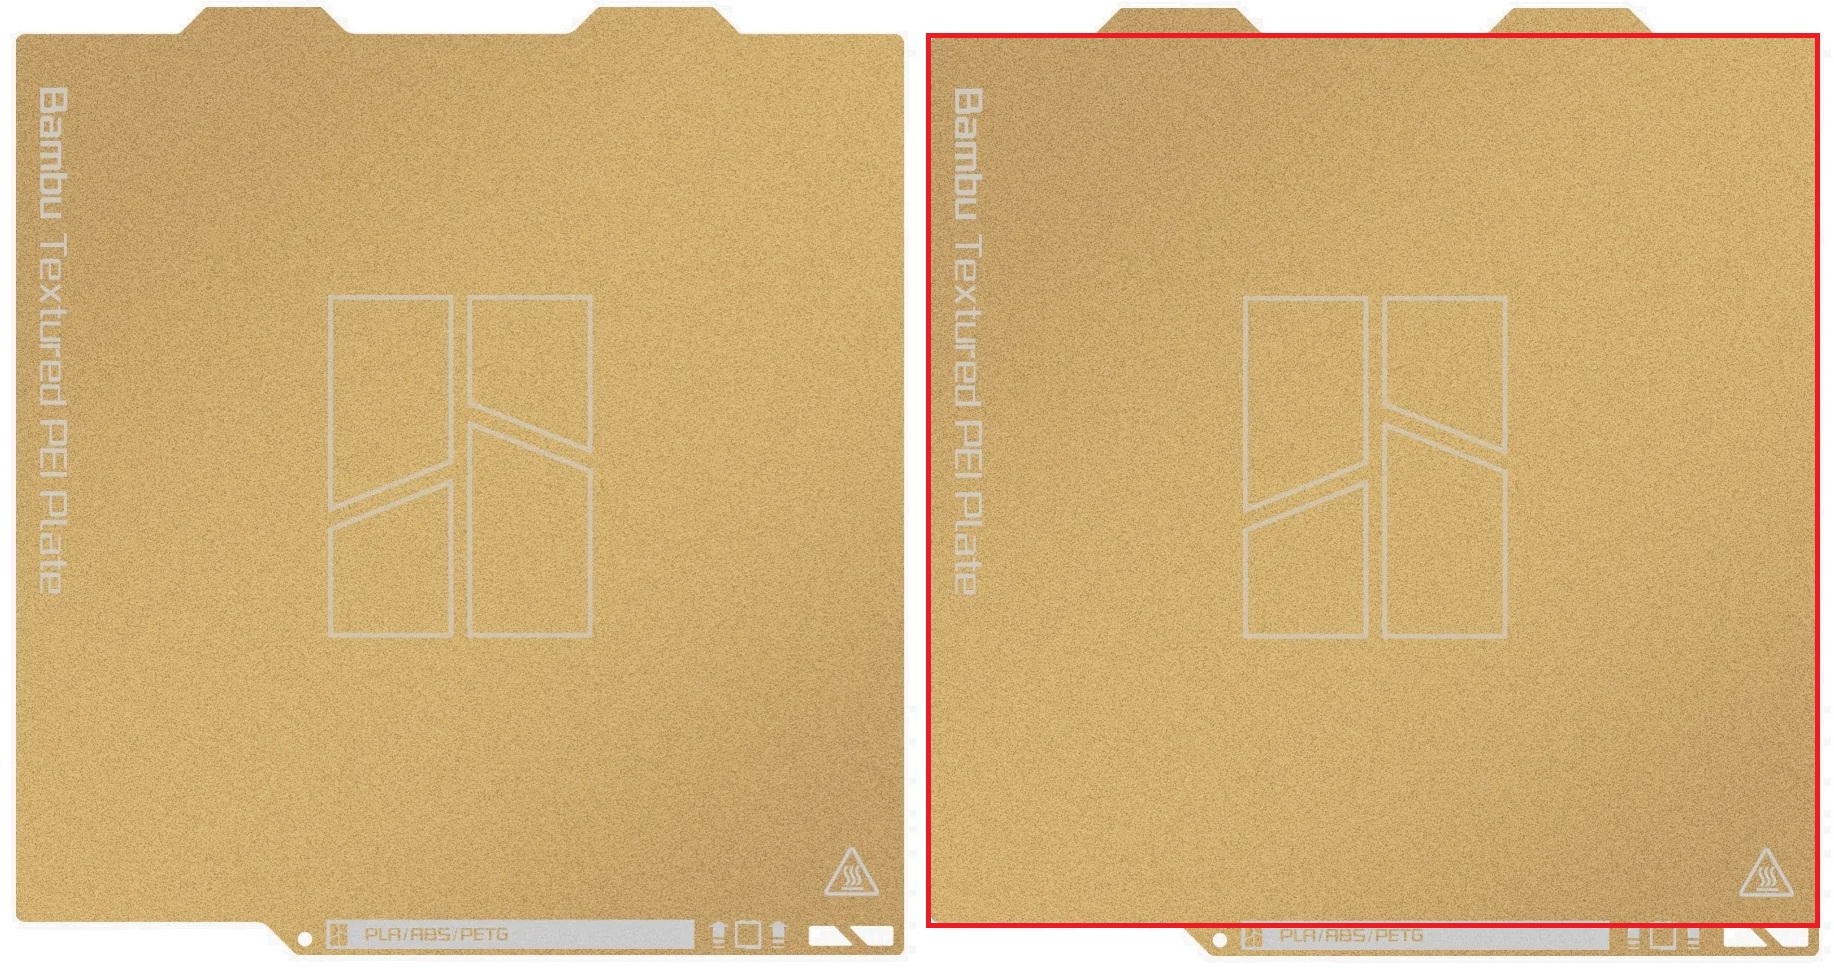
\includegraphics[width=0.7\textwidth]{PEIPlate}
  \textbf{\caption{PEI-пластина. На зображенні справа показано робочу зону}}
  \label{fig:PEI-plate}
\end{figure}

Робоча область PEI-пластини 18х18 см. Колір майже всіх PEI-пластин бронзово-золотистий. Отже, можна спробувати створити методи що шукають на зображенні проєкції квадратів, конкретний колір, або проєкції і колір одночасно.
Також, при використанні кольору як критерію пошуку, можна скористатись тим, що корпус даного 3D принтера в більшості місць білий.

Окрім роботи з значеннями пікселів для визначення кольору, можна скористатись тим, що робоча поверхня дуже контрастна з оточенням, корпусом принтера, і застосувати фільтр границь.

\section{Постановка задачі}
Програма має для вхідного зображення повернути 8 значень -- по дві координати чотирьох кутів столу/робочої області.

\section{Обрання методів розв'язку задачі}
Задачу розпізнавання об'єкту можуть виконати нейронні мережі, за наявності достатньої кількості розмічених зображень і функції втрат. 
Окрім нейронних мереж, можна застосувати ройові алгоритми, за умови наявності фітнес функції. 
Також, можна створити додатковий контекст, який гарантовано враховуватиме границі об'єктів та їх колір. Такий контекст можна подавати на вхід нейронних мереж чи ройових алгоритмів. 

\section{Створення методів отримання контексту}
\subsection{Отримання контексту з кольору пікселів}
З кольору пікселів можна створити контекст ввівши ідеальне значення кольору і допустимі відхилення. Доцільно це робити використавши HSV (трьохканальна система кольорів "Колірний тон, насиченість, яскравість"), а не RGB (трьохканальна система кольорів "Червоний, зелений, синій"), 
оскільки в HSV можна проігнорувати яскравість та враховувати лише колірний тон і насиченість.\\
Щоб отримати ідеальне значення кольорів столу і корпусу використано фотографію принтеру в типових умовах освітлення, отриману на камеру телефона.
\begin{figure}[H]
  \center
  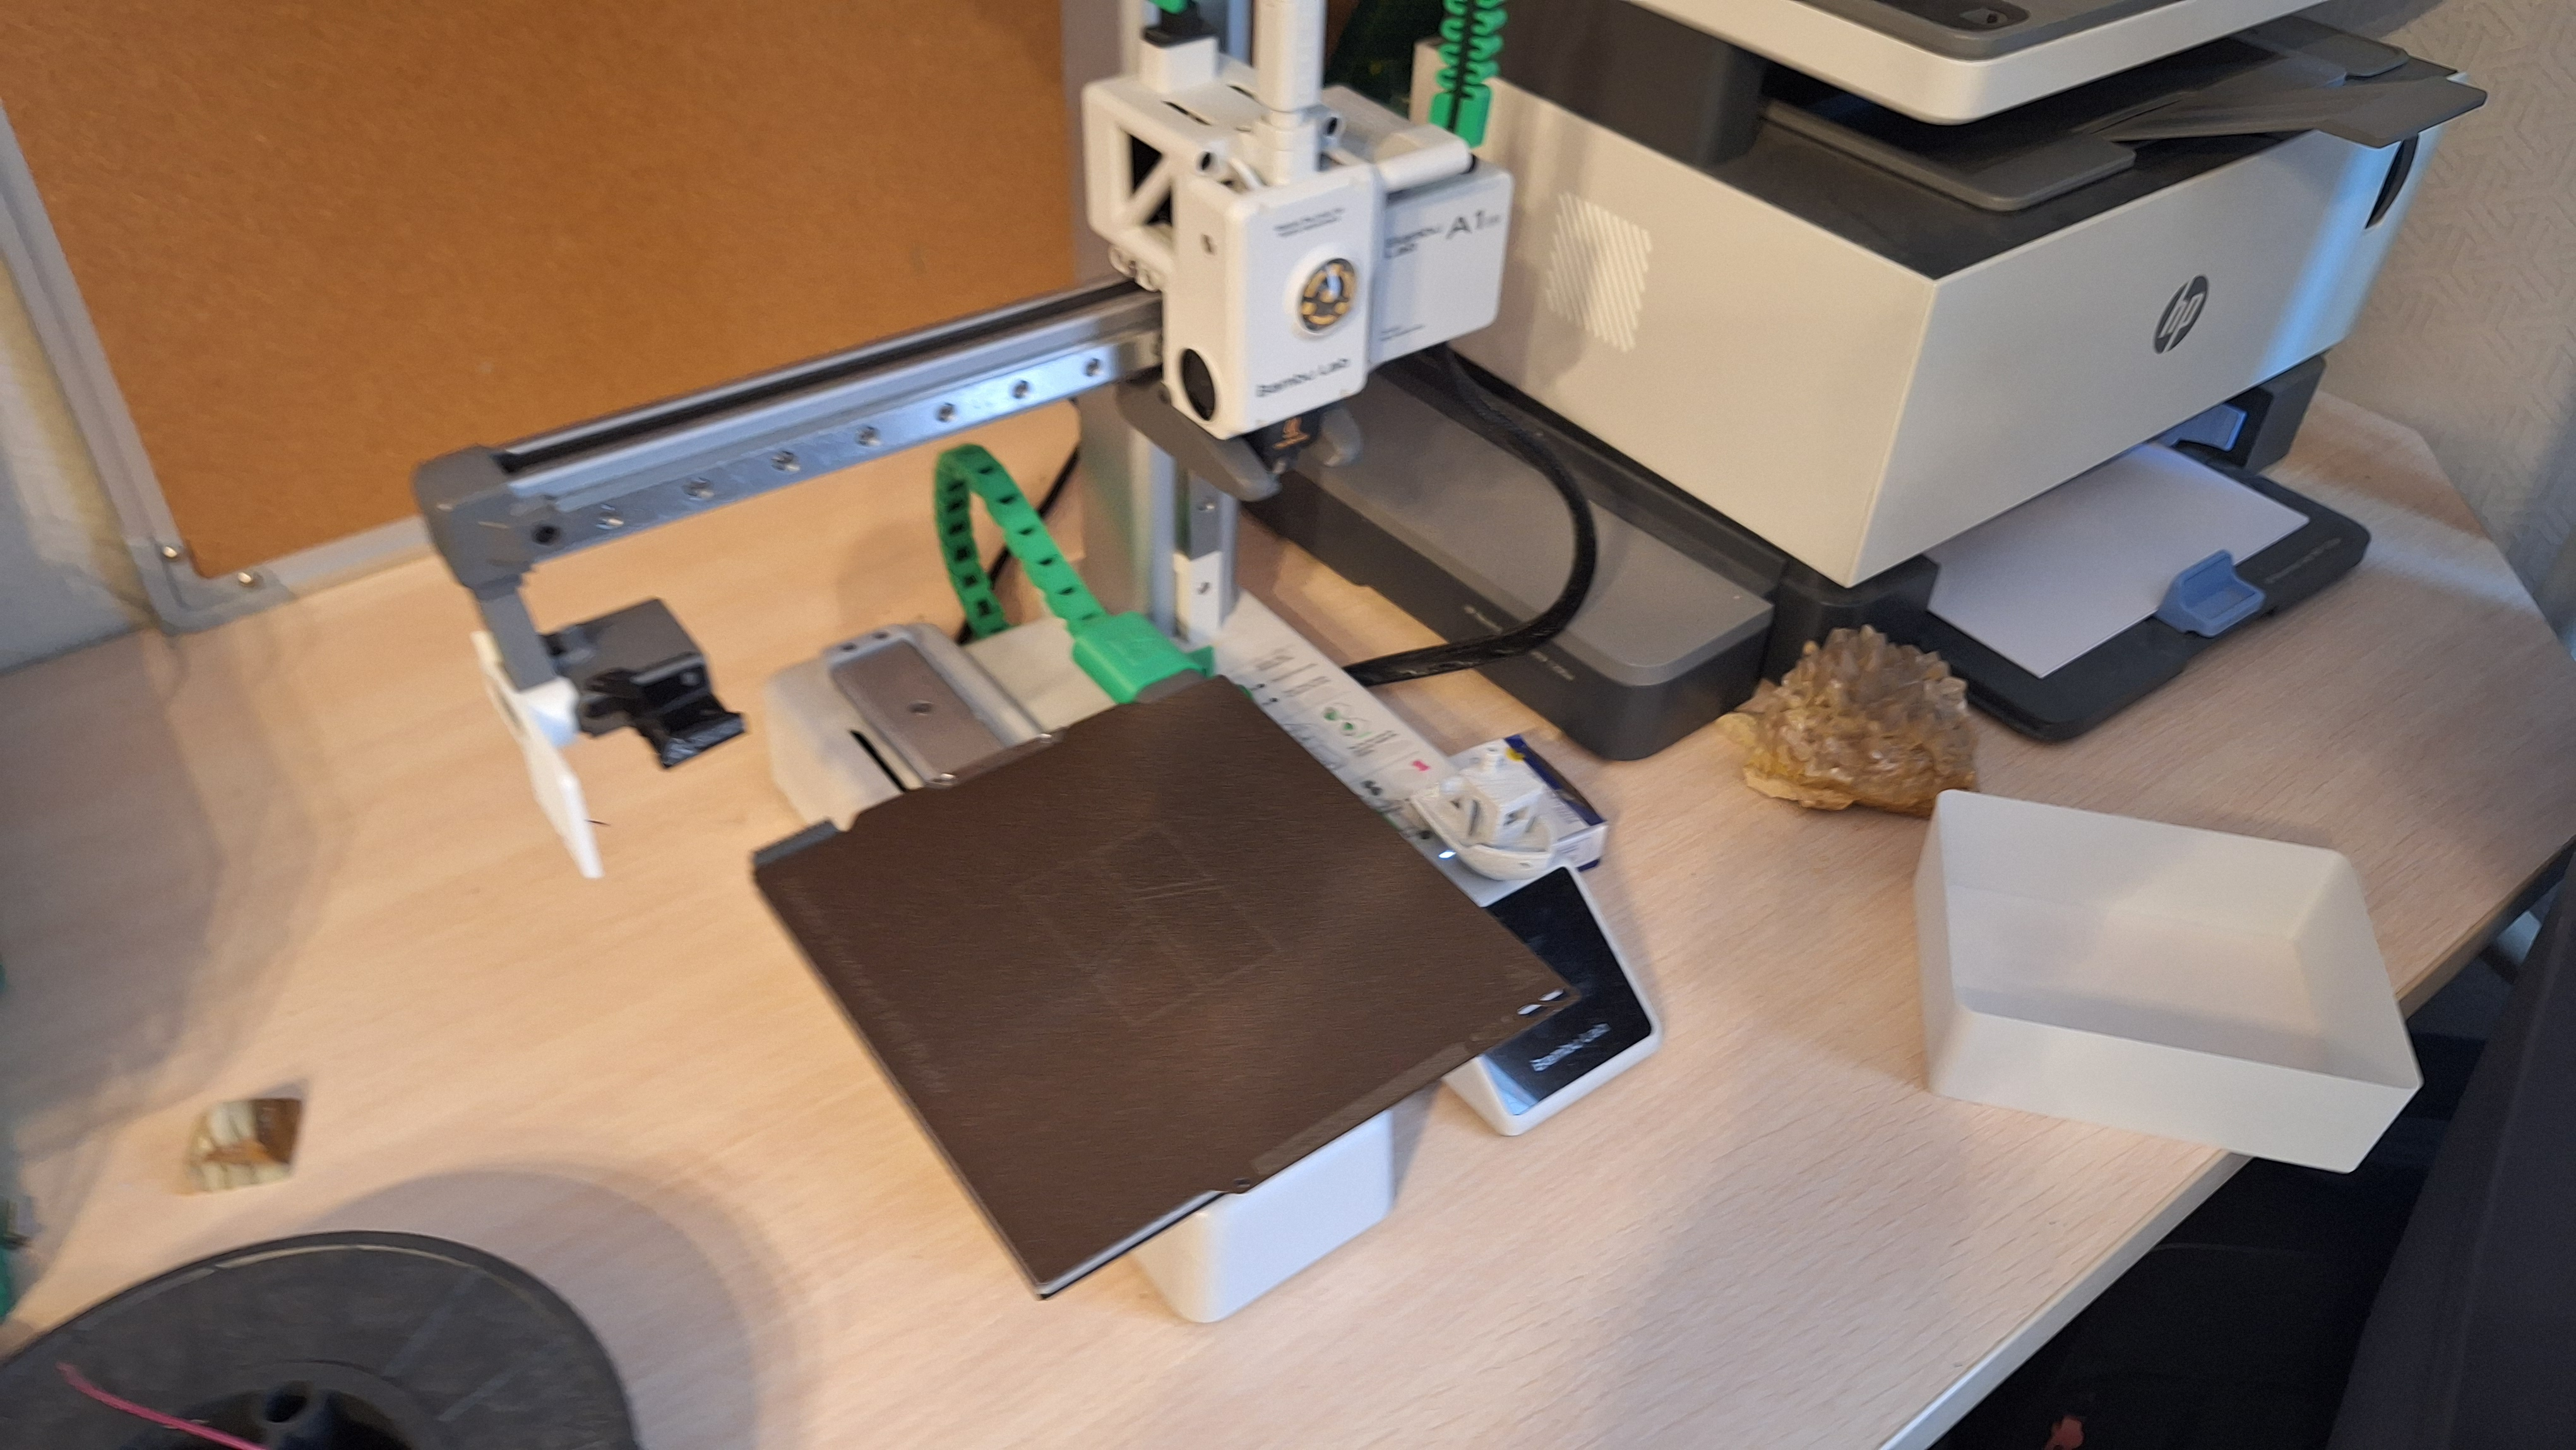
\includegraphics[width=0.7\textwidth]{DSExample1.jpg}
  \textbf{\caption{Зображення принтера отримане за допомогою камери телефона}}
  \label{fig:DSExample1}
\end{figure}

Отримані значення RGB: (89, 65, 55) для столу і (219, 208, 202) для корпусу. Після переходу в HSV отримано (0.05, 0.382, 0.349) і (0.0583, 0.078, 0.859) відповідно. 
Покладено допустимі відхилення тону кольору і насиченості в 0.1 для столу. 
Покладено що насиченість для корпусу має бути менша за 0.2, при будь-якому значенні тону. Дані правила застосовані для даного зображення.
\begin{figure}[H]
  \center
  \includegraphics[width=0.7\textwidth]{HSVContext1.png}
  \textbf{\caption{Перший набір правил застосований до зображення: правила для столу червоним, правила для корпусу білим}}
  \label{fig:HSVContext1}
\end{figure}

Застосування даних правил значно зменшило область пошуку столу, проте вона все ще залишалася великою. З порівняння зображень видно, що правила для столу спрацьовують для світлих ділянок, а правила для корпусу -- для темних. 
Щоб уникнути таких спрацювань, було додано правило на яскравість: для столу яскравість має бути меншою за середню на зображенні, а для корпусу -- більшою.
\begin{figure}[H]
  \center
  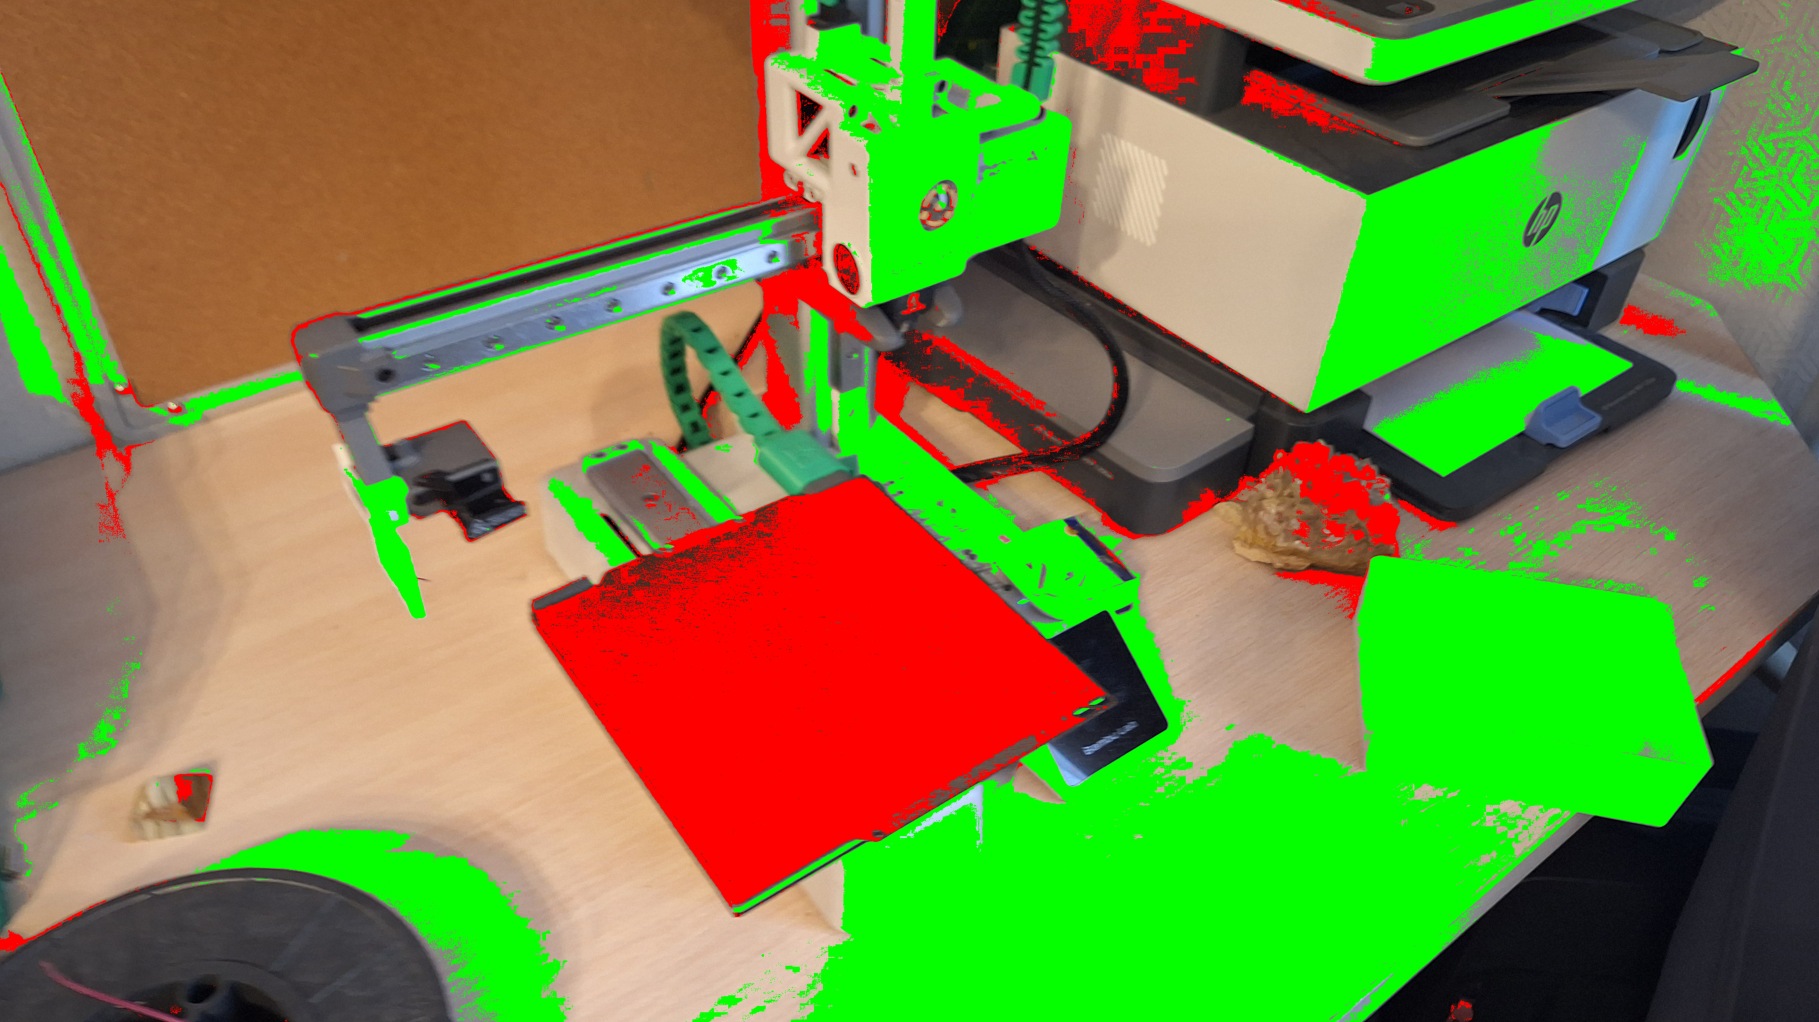
\includegraphics[width=0.7\textwidth]{HSVContext2.png}
  \textbf{\caption{Другий набір правил застосований до зображення}}
  \label{fig:HSVContext2}
\end{figure}

Дане розширення правил ще раз значно зменшило область пошуку. Проте, частина столу не фарбується в червоний, відповідно необхідно збільшити допустимі відхилення тону і насиченості. Допустимі відхилення збільшено вдвічі.
\begin{figure}[H]
  \center
  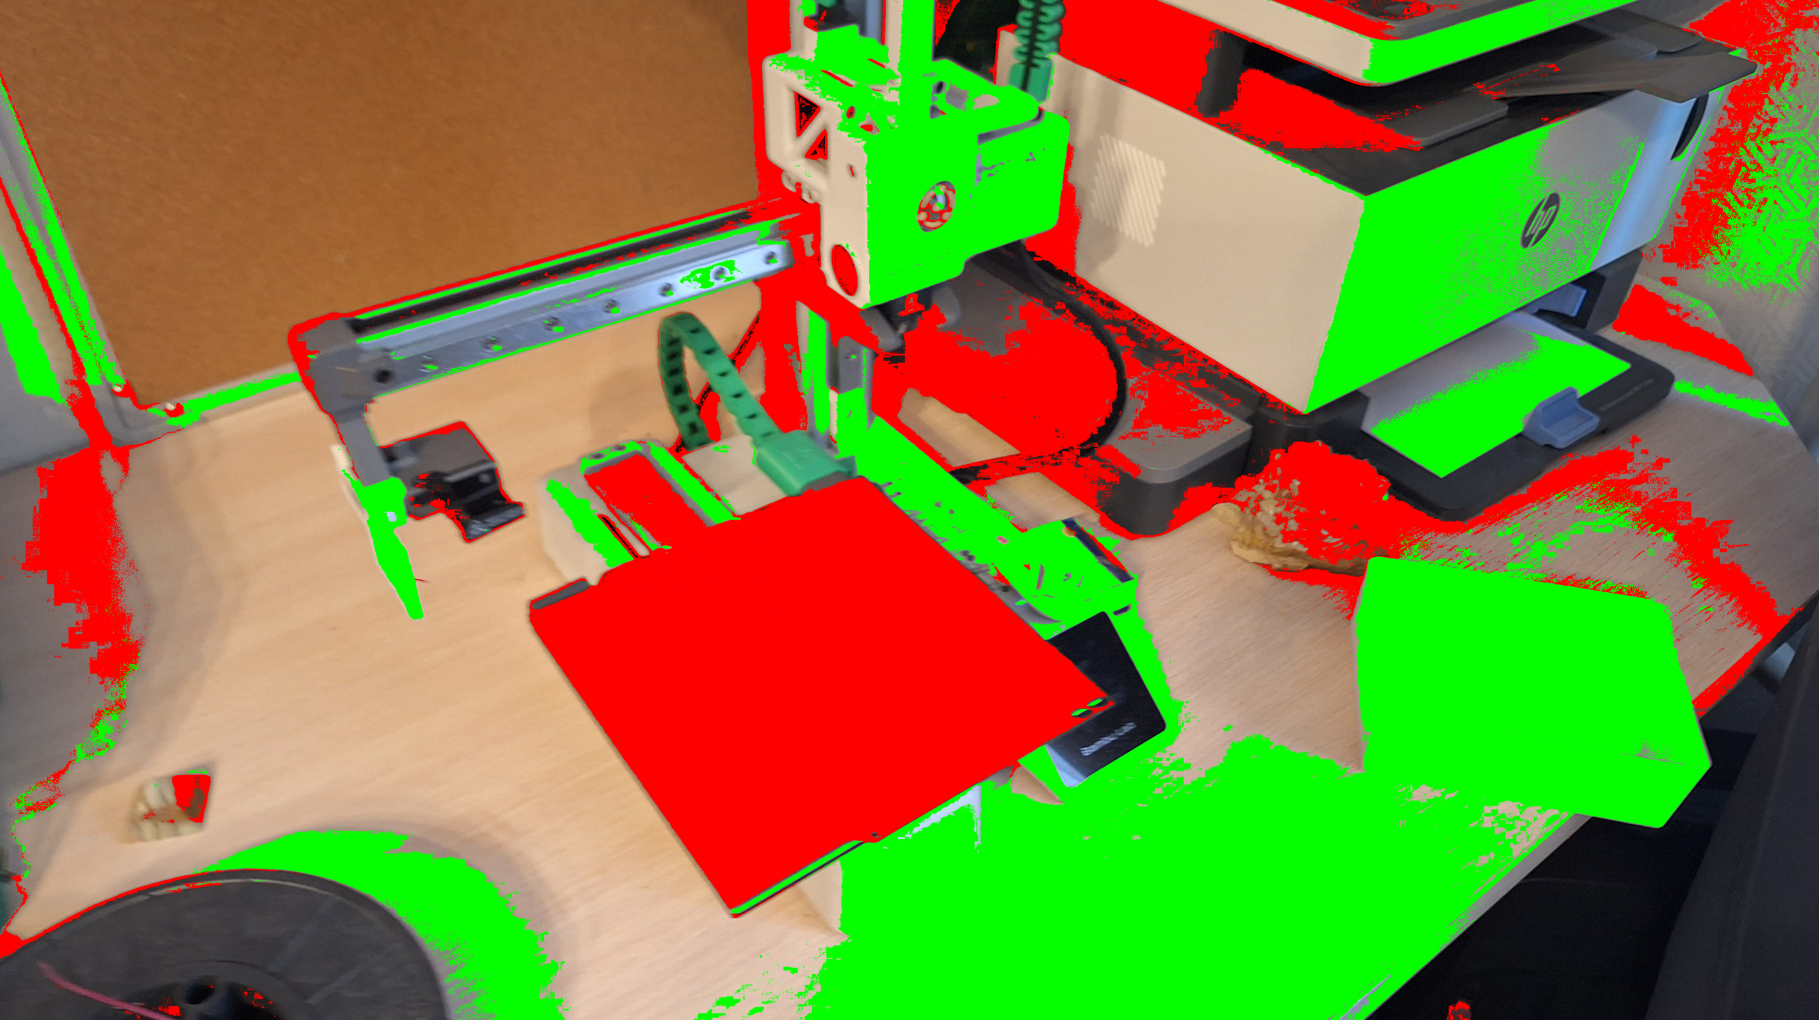
\includegraphics[width=0.7\textwidth]{HSVContext3.png}
  \textbf{\caption{Третій набір правил застосований до зображення}}
  \label{fig:HSVContext3}
\end{figure}

\subsection{Отримання границь, як джерел контексту}
Для отримання контексту у вигляді границь об'єктів необхідно застосувати матричний фільтр границь:
\[
kernel = 
\begin{pmatrix}
-1 & -1 & -1\\
-1 & 8 & -1\\
-1 & -1 &-1
\end{pmatrix}\]
Даний фільтр застосовано до різних зображень: оригінального, оригінального в HSV та, чорно-білого. 
Після чого було взято середнє всіх трьох каналів. 
Для кращого відображення границь, розмір зображення зменшено в 8 разів.

\begin{figure}[H]
  \center
  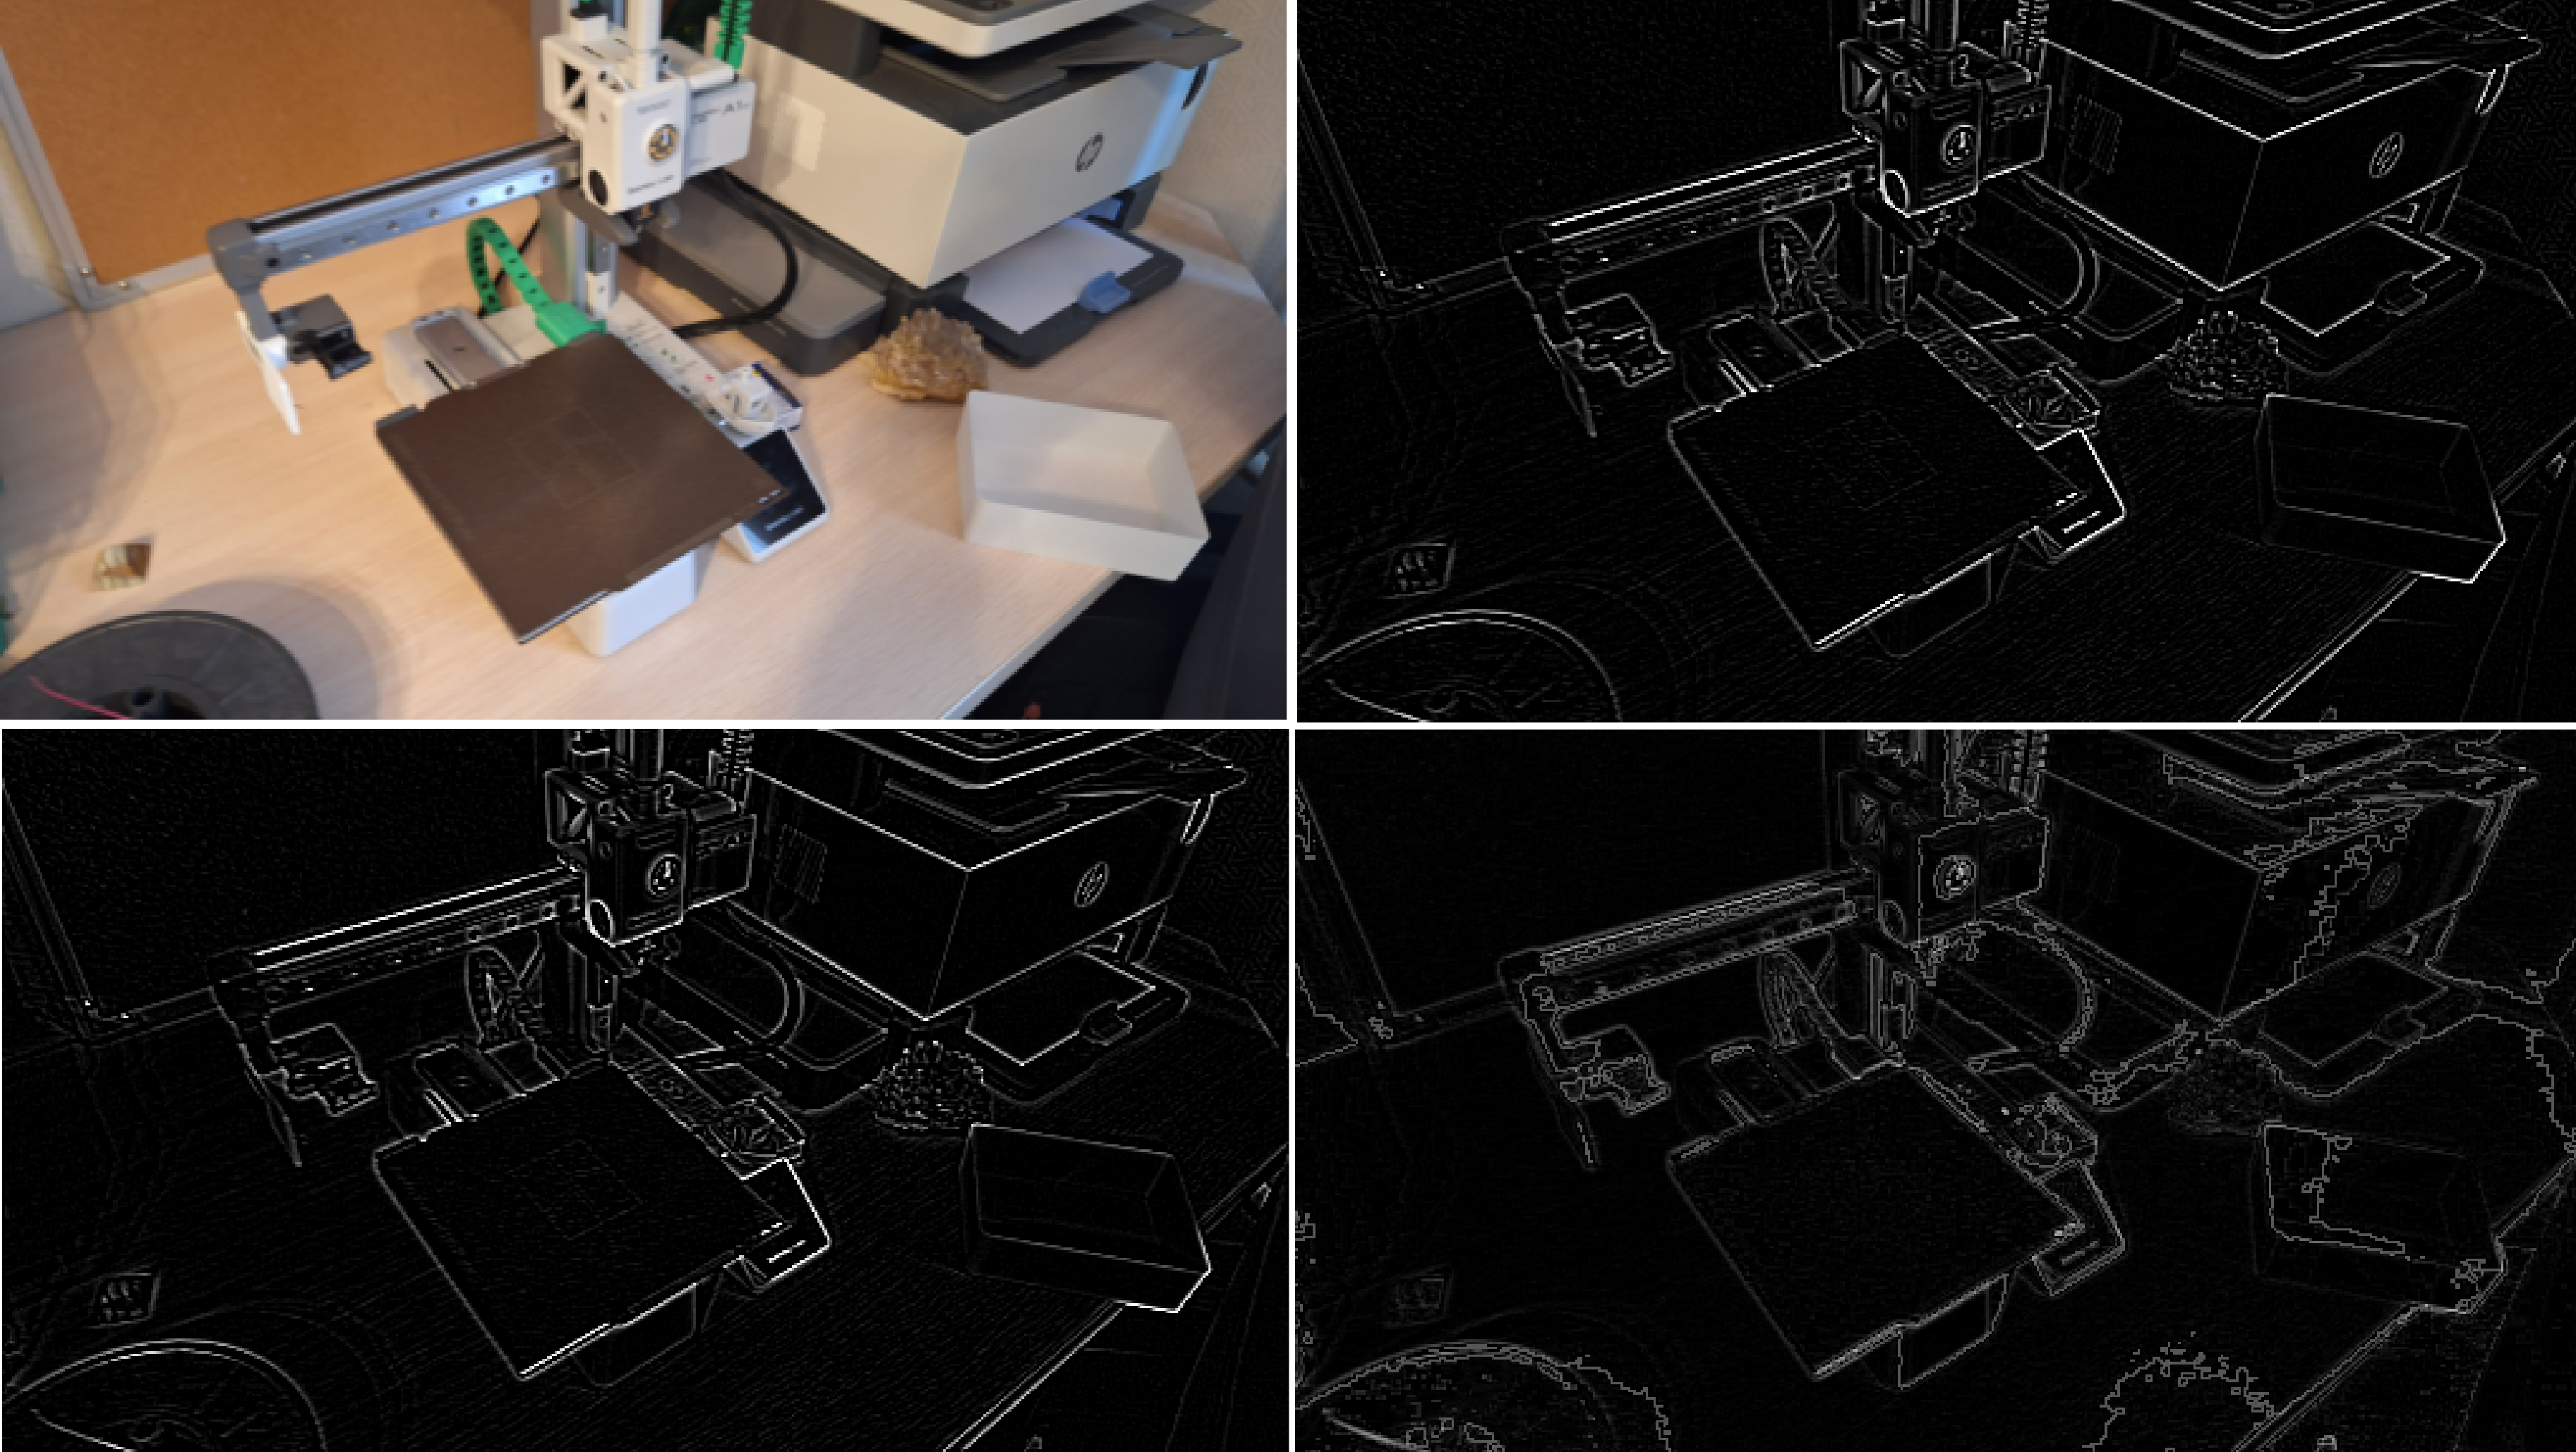
\includegraphics[width=\textwidth]{BordersRaw.png}
  \textbf{\caption{Перший ряд: оригінальне зображення, застосування фільтру до RGB, застосування фільтру до середнього значення каналів RGB, застосування фільтру до HSV}}
  \label{fig:BordersRaw}
\end{figure}

З зображень видно, що фільтр HSV має занадто нечіткі лінії щоб використовуватись далі.

Для утворення чітких границь, необхідно їх перетворити у бінарні значення 0 і 1. Один з більш простих способів такого перетворення -- прогове перетворення:
\[1, pixel \geq threshold\]
\[0, pixel < threshold\]

\begin{figure}[H]
  \center
  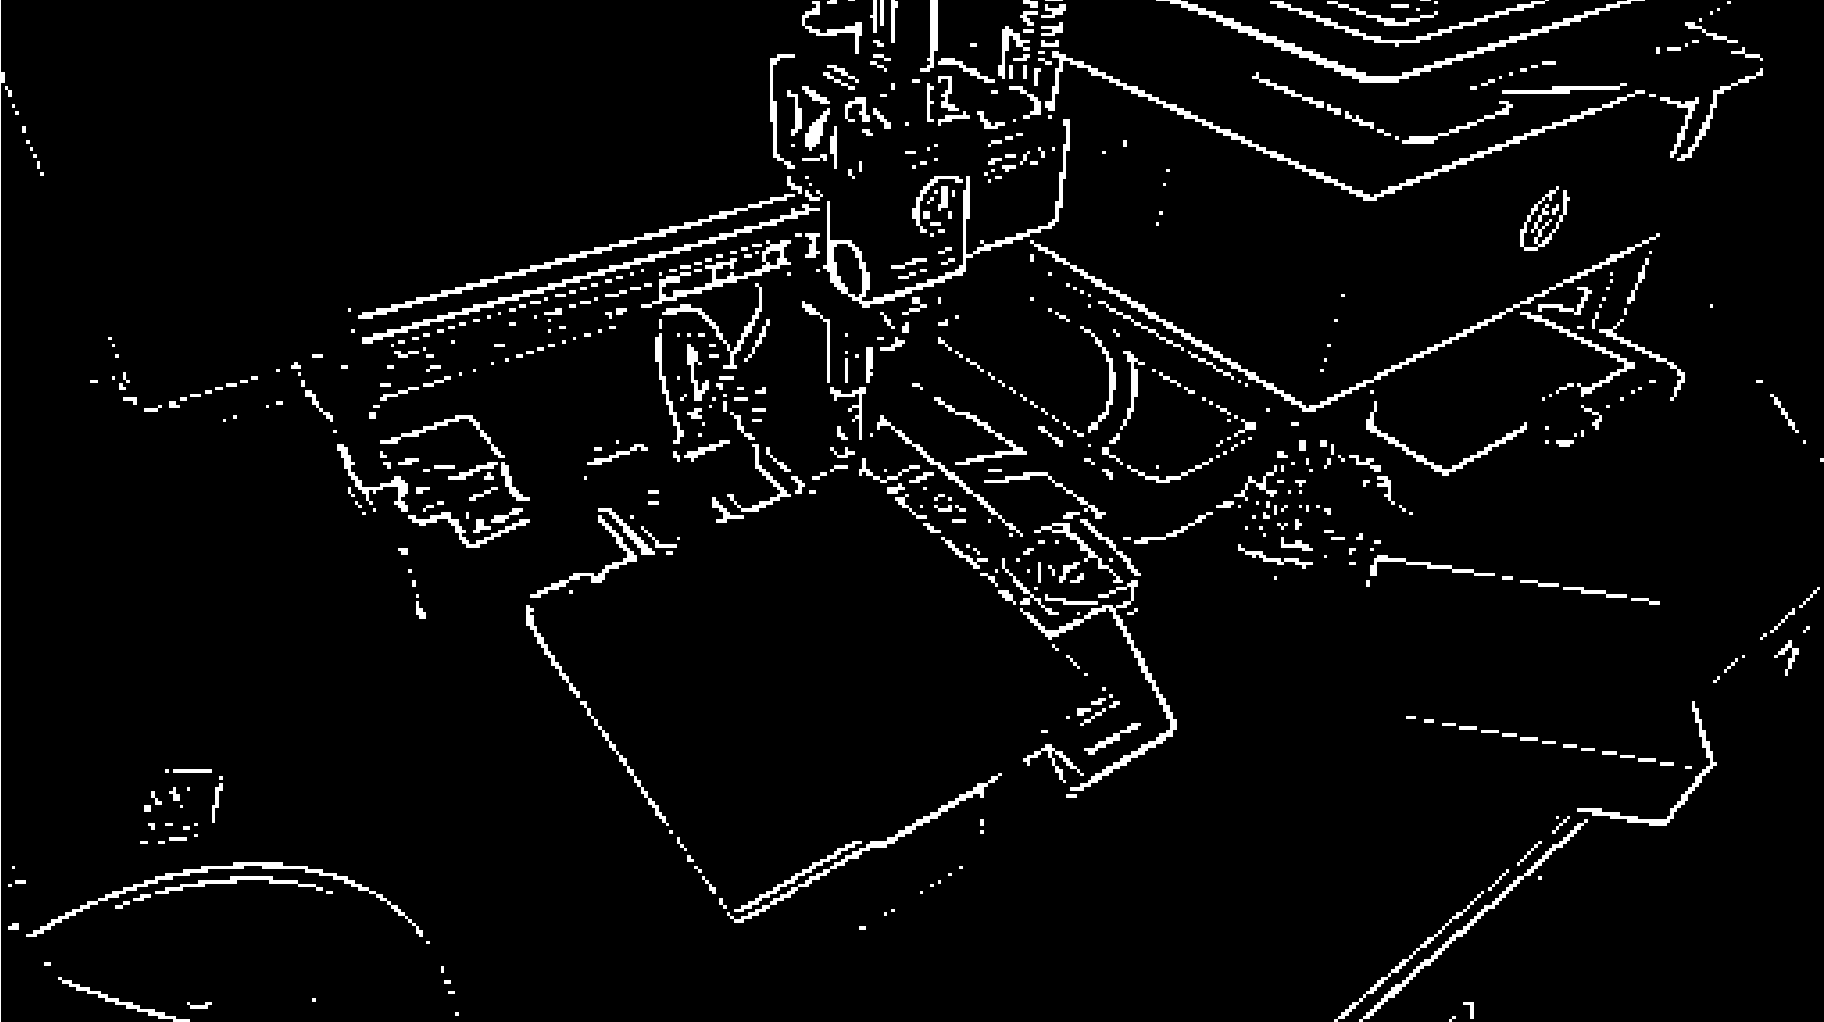
\includegraphics[width=0.7\textwidth]{BordersMasked.png}
  \textbf{\caption{Порогова бінаризація RGB границь з порогом 0.2}}
  \label{fig:BordersMasked}
\end{figure}

\subsection{Використання попередніх результатів розпізнання}
Нехай програма вже успішно змогла розмізнати стіл в попередньому моменті часу (наприклад на попередньому кадрі відео), тоді відомо масив точок що входили в регіон столу. Оскільки хід столу вперед-назад не перевищує розміру самого столу, то якась частина попереднього масиву точок мають опинитись в новому регіоні столу.
Можна впровадити простий критерій, що хоча б одна точка з попереднього регіону столу, має бути в новому регіоні столу.

Якщо попередні моменти часу відсутні, можна попросити людину, або більш потужний розпізнавач розпізнати початкове положення столу. 
У разі використання людини користувача/оператора, їй достатньо вказати якусь точку столу, щоб звичайний розпізнавач за цією точкою знайшов стіл на першому зображенні. 

\section{Створення фітнес-функції для оцінки чотирикутників}
\subsection{Загальні вимоги до фітнес-функцій}
Фітнес-функція має приймати на вхід вершини чотирикутника, окрім вершин функція може приймати значення вершин в попередній момент часу, початкову точку та константи пов'язані з оброблюваним зображенням.

\subsection{Функція оцінки квадратності чотирикутника}
Квадрат є паралелограмом, з більшості кутів огляду (викривленням лінзи можна знехтувати). 
Паралелограми мають наступні властивості: їх протилежні сторони рівні, їх протилежні сторони паралельні.

Оцінка рівності протележних сторін:
\[
\theta_E = \frac{(E_1-E_3)^2}{E_1+E_3} + \frac{(E_2-E_4)^2}{E_2+E_4}\text{, де }E_i\text{ -- довжина ребра.}
\]
В оцінці рівності протилежних сторін присутнє ділення на суму цих протилежних сторін, інакше оцінка буде працювати по-різному для різних довжин ребер.


Оцінка паралельності протележних сторін:
\[
\theta_\alpha = min^2(|\alpha_1-\alpha_3|, |\alpha_1+\alpha_3-2\pi|) + min^2(|\alpha_2-\alpha_4|, |\alpha_2+\alpha_4-2\pi|)\text{, де }\alpha_i\text{ -- кут нахилу ребра в радіанах.}
\]

Об'єднання оцінок рівності і паралельності протилежних сторін можна виконати безліччю методів. Простішими з них є сума і множення. 
Сума оцінок зберігає незалежність оцінок і дозволяє покращувати одну оцінку, навіть якщо інша занулена. Але сума потребує балансування оцінок, інакше алгоритми і моделі будуть намагатись оптимізувати оцінку з найбільшим абсолютним значенням. 
Множення не має необхідності балансування оцінок, проте має проблеми, якщо якась з оцінок занулюється. Щоб уникнути занулення, до оцінок можна додати невелику константу.

Оцінки об'єднані наступним чином:
\[
\theta_{\text{пар.}} = (\theta_E + c_1) \cdot (\theta_\alpha + c_2)\text{, де }c_i\text{ -- константи уникнення занулення, які необхідно визначити експериментально.}
\]

\subsection{Функція оцінки наявності границь поруч з сторонами чотирикутника}
Оскільки по периметру столу 3D принтера майже завжди знаходяться границі, можна рахувати кількість пікселів границі поруч з сторонами чотирикутника. 
Нехай "поруч"\ це "сторона проходить через піксель". 
Для визначення пікселів через які проходить відрізок існує алгоритм Брезенхейма. 
Загальне рівняння прямої через дві точки $(x_0, y_0)$, $(x_1, y_1)$:
\[
\frac{y-y_0}{y_1-y_0} = \frac{x-x_0}{x_1 - x_0}
\]
Алгоритм Брезенхейма, для всіх 8 напрямків прямої:
\begin{enumerate}
  \item p -- пустий масив точок;
  \item $\Delta x = |x_1 - x_0|$; $\Delta y = |y_1 - y_0|$;
  \item $sx = x_1 \geq x_0$; $sy = y_1 \geq y_0$;
  \item $x = x_0$; $y = y_0$;
  \item $D = argmax(\Delta x, \Delta y)$ -- домінантна вісь за якою відбуваються кроки, S -- інша вісь (X, Y = D, S або Y, X = D, S);
  \item $Error = floor(\Delta d / 2)$;
  \item Доки $d \neq d_1$:
  \item Записати (x, y) в p
  \item $Error = Error -  \Delta s$
  \item Якщо $Error < 0$, то: $s = s + ss$; $Error = Error + \Delta s$
  \item $d = d + sd$;
  \item Повернутись до "Доки";
  \item Записати $(x_1, y_1)$ в p;
  \item Повернути p.
\end{enumerate}

Для обрахунку кількості білих пікселів, алгоритм модифіковано наступним чином:
\begin{enumerate}
  \item p = 0;
  \item $\Delta x = |x_1 - x_0|$; $\Delta y = |y_1 - y_0|$;
  \item $sx = x_1 \geq x_0$; $sy = y_1 \geq y_0$;
  \item $x = x_0$; $y = y_0$;
  \item $D = argmax(\Delta x, \Delta y)$ -- домінантна вісь за якою відбуваються кроки, S -- інша вісь (X, Y = D, S, або Y, X = D, S);
  \item $Error = floor(\Delta d / 2)$;
  \item Доки $d \neq d_1$:
  \item $p = p + Image[x][y]$;
  \item $Error = Error -  \Delta s$
  \item Якщо $Error < 0$, то: $s = s + ss$; $Error = Error + \Delta s$
  \item $d = d + sd$;
  \item Повернутись до "Доки";
  \item $p = p + Image[x_1][y_1]$;
  \item Повернути p.
\end{enumerate}

Маючи алгоритм обрахунку кількості білих точок на відрізку, можна застосувати його для чотирьох сторін чотирикутника, сума результатів може бути функцією оцінки. 
Але, в такій реалізації оцінка штрафує за збільшення кількості білих точок. 
Нехай $B_4$ -- сума результатів роботи модифікованого алгоритму Брезенхейма, тоді:
\[
\theta = \frac{1}{B_4}
\]
оцінка яка винагороджує за кількість білих точок. Проте, така оцінка буде давати однакову винагороду за 1 білий піксель для чотирикутників з периметром 4 і з периметром 100.
Щоб цього уникнути, можна домножити на периметр:
\[
\theta_{B_4} = \frac{\sum\limits_{i=1}^{4}E_i}{B_4}
\]

\subsection{Функція оцінки внутрішніх границь}
Оскільки на зображенні цілком ймовірно може бути присутній інший паралелограм, то він може задовольнити попередні оцінки. 
Якщо цей паралелограм містить паралелограм столу, то навіть використання точок попереднього регіону столу може не допомогти. 
Якщо один паралелограм містить інший -- значить в ньому є білі пікселі границь внутрішнього паралелограму.

Можна побудувати оцінку, яка враховує кількість білих пікселів в чотирикутнику. Щоб побудувати таку оцінку необхідно побудувати алгоритм перевірки належності пікселя до чотирикутника.

Якщо точка знаходиться в чотирикутнику, промінь з цієї точки в будь-якому напрямку перетне чотирикутник. Якщо чотирикутник не опуклий і цей промінь перетне іншу сторону -- промінь має перетнути третю сторону щоб залишити чтоирикутник.
Таким чином, якщо промінь з точки в будь-якому напрямку перетинає сторони чотирикутника один чи три рази -- точка знаходиться в чотирикутнику.

Якщо хоча б один промінь з точки не перетинає жодну зі сторін чотирикутника -- точка лежить поза чотирикутником. Якщо ж перетинів парна ненульова кількість -- промінь спочатку заходив, а потім виходив з чотирикутника.

Таким чином: якщо для довільного променя кількість перетинів парна -- точка лежить поза чотирикутником, якщо непрна -- в середині. Для алгоритму використано промінь вздовж осі X:
\begin{enumerate}
  \item $inside = False$;
  \item Для кожної сторони:
  \item $x_i, y_i, x_j, y_j$ -- координати вершин сторони;
  \item Якщо промінь вздовж Х між $y_i$ та $y_j$ і якщо точка перетину з прямою сторони в середині сторони -- є перетин, $inside = not\ inside$;
  \item Після проходу по всім сторонам -- повернути $inside$.
\end{enumerate}

Маючи алгоритм належності пікселя до чотирикутника, можна побудувати алгоритм підрахунку білих точок в середині чотирикутника:
\begin{enumerate}
  \item $c = 0$;
  \item Для кожної білої точки на зображенні:
  \item Якщо точка в чотирикутнику -- $c = c+1$;
\end{enumerate}

Таким чином, оцінка внутрішніх границь має вигляд $\theta = c$. 
Але така оцінка не враховує розмір чотирикутника, для врахування розміру слід ділити на площу чотирикутника:
\[
\theta_c = \frac{c}{d_1 \cdot d_2 \cdot \cos(\beta)}\text{, де $d_i$ -- довжина діагоналі, $\beta$ -- кут між діагоналями}
\]

\subsection{Комбінація функцій оцінки у фінтес-функцію}
Одними з найбільш простих способів об'єднань оцінок є додавання і множення. 
Для того щоб уникнути балансування оцінок між собою, обрано множення:
\[
fitness = \theta_\text{пар.}\cdot (\theta_{B_4}+c_3)\cdot (\theta_c + c_4)\text{, де $c_i$ -- константи уникнення занулення, які треба визначити експериментально}
\]

\section{Створення первинного набору даних}
\subsection{Створення зображень}
Для набору даних на камеру телефона знято 50 фотографій принтера в однаковому довкіллі і при однаковому освітленні 
(різні умови довкілля не розглядаються для демонстрації роботи методів і зменшення часу на навчання моделей). 
Приклад однієї з таких фотографій на рисунку 2.2.

\subsection{Розстановка розмітки на зображеннях}
Розглянувши декілька програм для встановлення розмітки на зображеннях, обрано Label Studio як безкоштовний застосунок.
Для 50 зображень створено анотації з чотирикутниками.

\begin{figure}[H]
  \center
  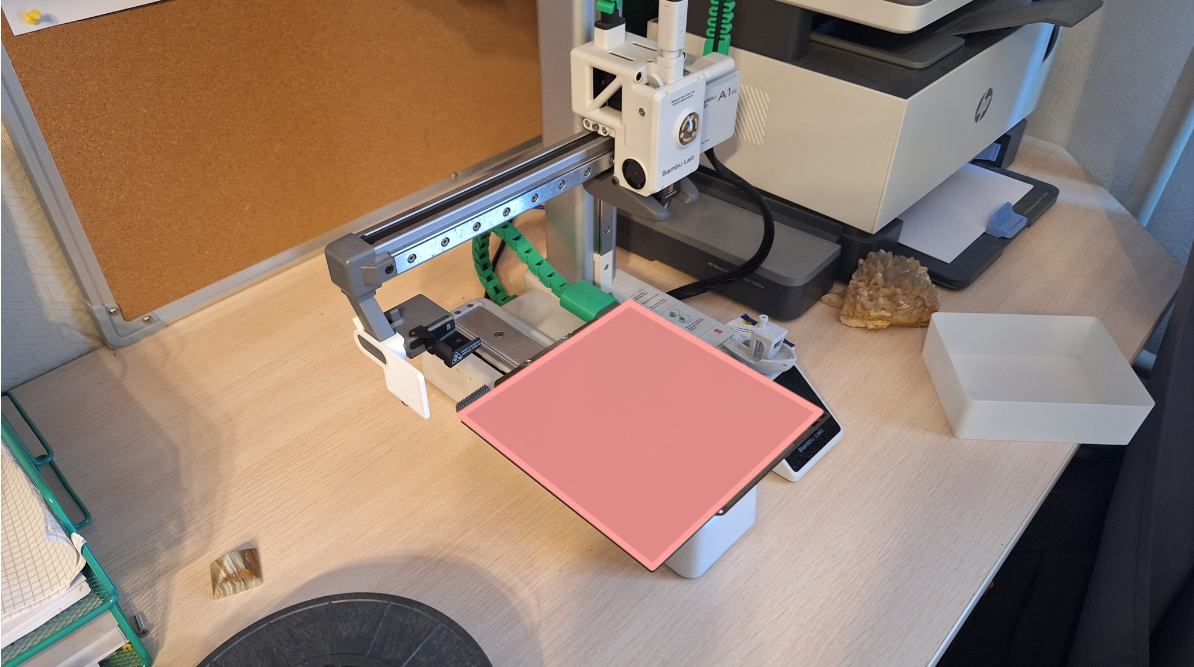
\includegraphics[width=0.7\textwidth]{LabelDemo.png}
  \textbf{\caption{Приклад розміченого зображення}}
  \label{fig:LabelDemo}
\end{figure}

\subsection{Збільшення варіативності набору даних}
Для збільшення варіативності набору даних, для кожного зображення створено 5 його версій: оригінальну, і чотири з випадковими шумом, поворотом та зміною кольору

TO DO!!!!!!


\chapter{Розробка програми}
\

\chapter{Висновки}

% Бібліографія
\begin{thebibliography}{9}
\bibitem{euler} Автор1. Назва книги. Видавництво, рік.
\bibitem{article} Автор2. Назва статті // Назва журналу. -- Рік. -- Том. -- С. 100-200.
\end{thebibliography}

\end{document}